\let\negmedspace\undefined
\let\negthickspace\undefined
\documentclass[journal,12pt,onecolumn]{IEEEtran}
\usepackage{cite}
\usepackage{amsmath,amssymb,amsfonts,amsthm}
\usepackage{algorithmic}
\usepackage{graphicx}
\graphicspath{{./figs/}}
\usepackage{textcomp}
\usepackage{xcolor}
\usepackage{txfonts}
\usepackage{listings}
\usepackage{enumitem}
\usepackage{mathtools}
\usepackage{gensymb}
\usepackage{comment}
\usepackage{caption}
\usepackage[breaklinks=true]{hyperref}
\usepackage{tkz-euclide} 
\usepackage{listings}
\usepackage{gvv}                                        
%\def\inputGnumericTable{}                                 
\usepackage[latin1]{inputenc}     
\usepackage{xparse}
\usepackage{color}                                            
\usepackage{array}                                            
\usepackage{longtable}                                       
\usepackage{calc}                                             
\usepackage{multirow}
\usepackage{multicol}
\usepackage{hhline}                                           
\usepackage{ifthen}                                           
\usepackage{lscape}
\usepackage{tabularx}
\usepackage{array}
\usepackage{float}
\newtheorem{theorem}{Theorem}[section]
\newtheorem{problem}{Problem}
\newtheorem{proposition}{Proposition}[section]
\newtheorem{lemma}{Lemma}[section]
\newtheorem{corollary}[theorem]{Corollary}
\newtheorem{example}{Example}[section]
\newtheorem{definition}[problem]{Definition}
\newcommand{\BEQA}{\begin{eqnarray}}
\newcommand{\EEQA}{\end{eqnarray}}
\newcommand{\define}{\stackrel{\triangle}{=}}
\theoremstyle{remark}
\newtheorem{rem}{Remark}

\begin{document}
\title{Assignment 1 : GATE PE 2018}
\author{ee25btech11056 - Suraj.N}
\maketitle
\renewcommand{\thefigure}{\theenumi}
\renewcommand{\thetable}{\theenumi}

\begin{enumerate}
 
\item``Going by the \_\_\_\_\_\_\_\_ that many hands make light work, the school \_\_\_\_\_\_\_\_ involved all the students in the task.''

\hfill{\brak{\text{GATE PE 2018}}} 

The words that best fill the blanks in the above sentence are 

\begin{enumerate}
\begin{multicols}{2}
\item principle,principal  \item principal,principle
\item principle,principle  \item principal,principal
\end{multicols}
\end{enumerate}

\item ``Her \_\_\_\_\_\_ should not be confused with miserliness; she is ever willing to assist those in need.'' 

\hfill{\brak{\text{GATE PE 2018}}} 

The word that best fills the blank in the above sentence is 

\begin{enumerate}
\begin{multicols}{4}
\item cleanliness  \item punctuality  \item frugality  \item greatness
\end{multicols}
\end{enumerate}

\item Seven machines take 7 minutes to make 7 identical toys. At the same rate, how many minutes would it take for 100 machines to make 100 toys? 

\hfill{\brak{\text{GATE PE 2018}}}

\begin{enumerate}
\begin{multicols}{4}
\item1  \item7  \item100  \item700 
\end{multicols}
\end{enumerate}

\item A rectangle becomes a square when its length and breadth are reduced by 10 m and 5 m, respectively. During this process, the rectangle loses $650 \ \mathrm{m}^2$ of area. What is the area of the original rectangle in square meters? 

\hfill{\brak{\text{GATE PE 2018}}} 

\begin{enumerate}
\begin{multicols}{4}
\item 1125   \item 2250  \item 2924  \item 4500
\end{multicols}
\end{enumerate}

\item A number consists of two digits. The sum of the digits is 9. If 45 is subtracted from the number, its digits are interchanged. What is the number? 

\hfill{\brak{\text{GATE PE 2018}}}\begin{enumerate}

\begin{multicols}{4}
\item 63  \item 72  \item 81 \item 90    
\end{multicols}
\end{enumerate}

\item For integers $a, b$ and $c$, what would be the minimum and maximum values respectively of $a + b + c$ if $\log |a| + \log |b| + \log |c| = 0$? 

\hfill{\brak{\text{GATE PE 2018}}}

\begin{enumerate}
\begin{multicols}{4}
\item -3 and 3 \item -1 and 1 \item -1 and 3 \item 1 and 3
\end{multicols}
\end{enumerate}

\pagebreak

\item Given that $a$ and $b$ are integers and $a + a^2b^3$ is odd, which one of the following statements is correct? 

\hfill{\brak{\text{GATE PE 2018}}}

\begin{enumerate}
\begin{multicols}{2}
\item $a$ and $b$ are both odd \item $a$ and $b$ are both even
\item $a$ is even and $b$ is odd \item $a$ is odd and $b$ is even
\end{multicols}
\end{enumerate}

\item From the time the front of a train enters a platform, it takes 25 seconds for the back of the train to leave the platform, while travelling at a constant speed of 54 km/h. At the same speed, it takes 14 seconds to pass a man running at 9 km/h in the same direction as the train. What is the length of the train and that of the platform in meters, respectively? 

\hfill{\brak{\text{GATE PE 2018}}}

\begin{enumerate}
\begin{multicols}{2}
\item 210 and 140 \item 162.5 and 187.5
\item 245 and 130 \item 175 and 200
\end{multicols}
\end{enumerate}

\item Which of the following functions describe the graph shown in the below figure?

\hfill{\brak{\text{GATE PE 2018}}}

\begin{figure}[h!]
  \centering
  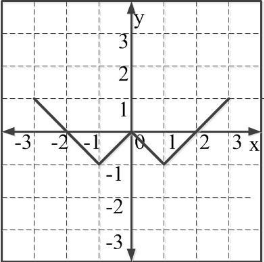
\includegraphics[width=0.4\columnwidth]{figs/pic1.png} 
  \caption*{}
  \label{fig:Q9}
\end{figure}
  
\begin{center}
\begin{enumerate}
\begin{multicols}{2}

 \item $y = ||x| + 1| - 2$ \item $y = ||x| - 1| - 1$
 \item $y = ||x| + 1| - 1$ \item $y = ||x - 1| - 1|$

\end{multicols}
\end{enumerate}
\end{center}

\pagebreak

\item Consider the following three statements:

\begin{enumerate}	
\item Some roses are red.
\item All red flowers fade quickly.
\item Some roses fade quickly.
\end{enumerate}

\noindent
Which of the following statements can be logically inferred from the above statements?

\hfill{\brak{\text{GATE PE 2018}}}

\begin{enumerate}
\item If \brak{i} is true and \brak{ii} is false, then \brak{iii} is false.
\item If \brak{i} is true and \brak{ii} is false, then \brak{iii} is true.
\item If \brak{i} and \brak{ii} are true, then \brak{iii} is true.
\item If \brak{i} and \brak{ii} are false, then \brak{iii} is false.
\end{enumerate}

\item The Taylor series expansion of the function,

\hfill{\brak{\text{GATE PE 2018}}}

\begin{align*}
{\Large f(x) = \frac{-1}{1+x}}
\end{align*}

\noindent
around $x = 0$ \brak{\text{up to 4th order term}} is:

\begin{enumerate}
\item $ 1 + x + x^2 + x^3 + x^4$
\item $ -1 + x - x^2 + x^3 - x^4$
\item $ -1 - x + x^2 - x^3 + x^4$
\item $ -1 + x - 2x^2 + 3x^3 - 4x^4$
\end{enumerate}

\item The inverse of the matrix $\myvec{ 1 & 3 \\ 1 & 2}$ is, 

\hfill{\brak{\text{GATE PE 2018}}}

\begin{enumerate}
\begin{multicols}{4}
\item $\myvec{ 2 & 3 \\ 1 & 1 }$ 
\item $\myvec{ -2 & 1 \\ 3 & -1}$ 
\item $\myvec{ -2 & 3 \\ 1 & -1}$ 
\item $\myvec{ 2 & -3 \\ -1 & 1 }$
\end{multicols}
\end{enumerate}

\item The line integral of a vector function $\vec{F}(\vec{r})$ over a curve $C$ in a simply connected domain $D$ in space, is defined by: 

\hfill{\brak{\text{GATE PE 2018}}}

\begin{align*}
\int_C \vec{F}(\vec{r}) \cdot d\vec{r} = \int_C (F_1 dx + F_2 dy + F_3 dz)
\end{align*}

The line integral is independent of path in $D$. $F_1$, $F_2$, and $F_3$ are continuous, and have continuous first partial derivatives in $D$. $C'$ is a closed curve in $D$.\\

\noindent
Which one of the following is \textbf{NOT ALWAYS} true in domain $D$?

\begin{enumerate}
\begin{multicols}{2}
\item $\nabla \times \vec{F} = \vec{0}$  \item $\nabla \cdot \vec{F} = 0$ \hspace{2em}
\item $\oint_{C'} \vec{F}(\vec{r}) \cdot d\vec{r} = 0$  \item $\vec{F} \times \vec{F} = \vec{0}$
\end{multicols}
\end{enumerate}

\item Which one of the following is the integrating factor \brak{IF} for the differential equation, $(\cos^2 x)\dfrac{dy}{dx} + y = \cos x$ ? 

\hfill{\brak{\text{GATE PE 2018}}}

\begin{enumerate}
\begin{multicols}{2}
\item $e^{\tan x}$  \item $e^{\cos x}$ 
\item $e^{-\tan x}$  \item $e^{\sin x}$
\end{multicols}
\end{enumerate}

\pagebreak

\item A phase diagram of a black oil is shown in the figure \brak{\text{Y is the critical point}}.

\hfill{\brak{\text{GATE PE 2018}}}

\begin{figure}[h!]
  \centering
  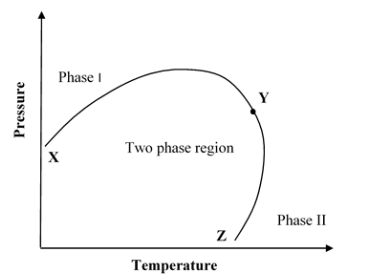
\includegraphics[width=0.6\columnwidth]{figs/pic2.png} 
   \caption*{}
  \label{fig:Q15}
\end{figure}

\noindent
Match the following:\\\\

\begin{tabular}{ll}
P. Curve XY & I. Dew point curve\\
Q. Curve YZ & II. Single phase liquid\\
R. Phase I  & III. Bubble point curve\\
S. Phase II &  IV. Single phase gas
\end{tabular}

\begin{enumerate}
\begin{multicols}{2}
\item P-I, Q-III, R-II, S-IV \item P-III, Q-I, R-II, S-IV
\item P-III, Q-I, R-IV, S-II \item P-I, Q-II, R-III, S-IV
\end{multicols}
\end{enumerate}


\item Match the following chemicals to their respective oilfield applications:

\hfill{\brak{\text{GATE PE 2018}}}\\\\

\begin{tabular}{ll}
P. Hydrate inhibitor & I. Formaldehyde\\
Q. Well stimulation & II. Xanthan gum\\
R. Drilling fluid biocide & III. Methanol\\
S. Viscosifier & IV. Hydrochloric acid\\\\
\end{tabular}

\begin{enumerate}
\begin{multicols}{2}
\item P-IV, Q-III, R-II, S-I \item P-III, Q-I, R-IV, S-II
\item P-I, Q-III R-IV, S-II \item P-III, Q-IV, R-I, S-II 
\end{multicols}
\end{enumerate}

\pagebreak

\item The CH4-hydrate equilibrium curve \brak{\text{dashed}} and CO2-hydrate equilibrium curve \brak{\text{solid}} on a pressure-temperature plane above 0{\degree}C are shown in the figure. The two curves divide the plane in four non-overlapping regions. In which region are CO2-hydrates stable and CH4-hydrates unstable?

\hfill{\brak{\text{GATE PE 2018}}}

\begin{figure}[h!]
  \centering
  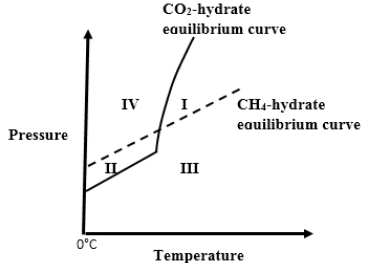
\includegraphics[width=0.5\columnwidth]{figs/pic3.png} 
   \caption*{}
  \label{fig:Q17}
\end{figure}

\begin{enumerate}
\begin{multicols}{4}
\item I  \item II  \item III  \item IV 
\end{multicols}
\end{enumerate}

\item Plot of ratio of pressure to gas compressibility factor \brak{P/Z} vs. cumulative gas production
\brak{Gp} for a gas reservoir \brak{\text{represented by solid curve in the figure}} was shown to a reservoir
engineering student.

\hfill{\brak{\text{GATE PE 2018}}}

\begin{figure}[h!]
  \centering
  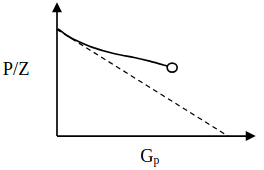
\includegraphics[width=0.4\columnwidth]{figs/pic4.png} 
   \caption*{}
  \label{fig:Q18}
\end{figure}

\noindent
The student made the following statements:

\begin{enumerate}
\item A water aquifer is attached to this gas reservoir.
\item P/Z vs. Gp curve must always be a straight line for water encroachment in a gas reservoir.
\item The ultimate gas recovery is diminished due to water encroachment.
\end{enumerate}

Which of the above statements are \textbf{TRUE}?


\begin{enumerate}
\begin{multicols}{4}
\item Only I and II \item Only II and III \item Only I and III \item I, II, and III
\end{multicols}
\end{enumerate}

\pagebreak

\item  Waste water from oil industry consists of oil in free and emulsified forms. The oil in the
free form can be recovered by:

\hfill{\brak{\text{GATE PE 2018}}}

\begin{enumerate}
\begin{multicols}{2}
\item Aerated lagoons
\item Trickling filters
\item Gravity separators
\item Biological oxygen pond
\end{multicols}
\end{enumerate}

\noindent
\item A reservoir model consisting of two porous matrices M and N, separated by a fracture, is shown in the figure. The matrices are strongly water-wet and are saturated with oil of specific gravity 0.8. Water is injected only in the fracture at injection well A. If the Reynolds number for the flow in the fracture conduit is assumed to be less than unity, which one of the following force will dominate oil recovery from the porous matrix M during the water-flood operation?

\hfill{\brak{\text{GATE PE 2018}}}

\begin{figure}[h!]
  \centering
  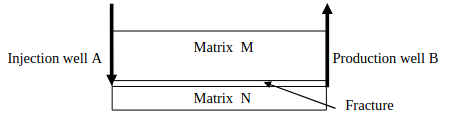
\includegraphics[width=0.6\columnwidth]{figs/pic5.png} 
   \caption*{}
  \label{fig:Q20}
\end{figure}

\begin{enumerate}
\begin{multicols}{2}
\item Capillary force \item Gravity force
\item Viscous force \item Inertial force
\end{multicols}
\end{enumerate}

\item A fractional flow curve is given for a core for which the irreducible water saturation is 0.2 and the residual oil saturation is 0.3. The initial water saturation in the core is 0.3. If Welge's method is applied to find the breakthrough saturation and fraction flow of water at breakthrough, which point should be used in the figure to draw a tangent line to the
fractional flow curve.

\hfill{\brak{\text{GATE PE 2018}}}

\begin{figure}[h!]
  \centering
  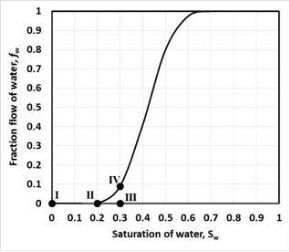
\includegraphics[width=0.3\columnwidth]{figs/pic6.png} 
   \caption*{}
  \label{fig:Q21}
\end{figure}

\begin{enumerate}
\begin{multicols}{4}
\item I \item II \item III \item IV
\end{multicols}
\end{enumerate}

\pagebreak

\item Which one of the following curves represents behavior of oil phase viscosity as a function of pressure in the reservoir \brak{\text{where, Pb is the bubble point pressure of oil}}?

\hfill{\brak{\text{GATE PE 2018}}}

\begin{figure}[h!]
  \centering
  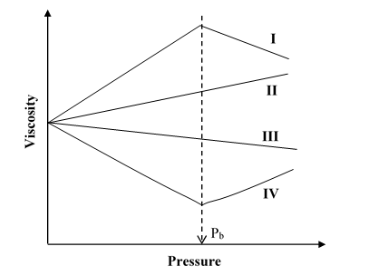
\includegraphics[width=0.6\columnwidth]{figs/pic7.png} 
   \caption*{}
  \label{fig:Q22}
\end{figure}

\begin{enumerate}
\begin{multicols}{4}
\item Curve I  \item Curve II \item Curve III \item Curve IV
\end{multicols}
\end{enumerate}

\item Pick out the \textbf{INCORRECT} statement.

\hfill{\brak{\text{GATE PE 2018}}}

\begin{enumerate}
\item Flash point is always lower than fire point.
\item Pour point of lube oil can be reduced by removing the wax from it.
\item Fracturing is a well stimulation technique.
\item Coal bed methane typically contains more than 60\% $CO_2$.
\end{enumerate}

\item Which one of the following phenomena encountered during flooding is desirable for
increasing oil recovery from a reservoir?

\hfill{\brak{\text{GATE PE 2018}}}

\begin{enumerate}
\begin{multicols}{2}
\item Viscous fingering \item Formation damage
\item Increase in mobility ratio \item Decrease in capillary pressure
\end{multicols}
\end{enumerate}

\item $CO_2$ foams are used for enhanced oil recovery due to which of the following reasons?

\hfill{\brak{\text{GATE PE 2018}}}

\begin{enumerate}
\item It can be used for $CO_2$ sequestration
\item $CO_2$ can exist in the form of a dense fluid at reservoir conditions
\item $CO_2$ can convert to hydrocarbon at the reservoir temperature and pressure
\item Solubility of $CO_2$ in oil is higher compared to gases like $N_2$
\end{enumerate}

\begin{enumerate}
\begin{multicols}{2}
\item Only I, II, and III \item Only I, II, and IV
\item Only II, III, and IV \item Only I, III, and IV
\end{multicols}
\end{enumerate}

\pagebreak

\item Which one of the following is FALSE about a typical offshore deepwater oil spill?

\hfill{\brak{\text{GATE PE 2018}}}

\begin{enumerate}
\item Using boom boats to prevent spilled oil from spreading
\item Allowing the spill to reach the shore before clearing
\item Burning of spilled oil
\item Using a skimmer to collect the oil
\end{enumerate}

\item Which one of these methods is NOT commonly used to deal with the problem of soil
contamination by oil spillage?\hfill{\brak{\text{GATE PE 2018}}}
\begin{enumerate}
\item Biodegradation
\item Leaching out the oil
\item Soil recycling
\item Using rain water to wash the contaminants
\end{enumerate}

\item The factor on which the selection of an offshore platform for the reservoir does \textbf{NOT}
depend:

\hfill{\brak{\text{GATE PE 2018}}}

\begin{enumerate}
\item Water depth
\item Reservoir fluid properties
\item Sea bed conditions
\item Best case weather forecast
\end{enumerate}

\item Which one of the following options is correct about the effects of steam stimulation in increasing the oil production rate?

\hfill{\brak{\text{GATE PE 2018}}}

\begin{enumerate}
\item Reduces the oil viscosity
\item Increases the formation damage
\item Reduces the interfacial tension
\item Increases the oil viscosity
\end{enumerate}

\begin{enumerate}
\item Only I and II
\item Only II and III
\item Only III and IV
\item Only I and III
\end{enumerate}

\item  Which one of the following is \textbf{INCORRECT} about oil based drilling muds?

\hfill{\brak{\text{GATE PE 2018}}}

\begin{enumerate}
\item Good rheological properties at higher temperatures \brak{\text{as high as $250{\degree}C$.}}
\item Effective against corrosion
\item Detection of gas kick is difficult
\item Less inhibitive than water based muds
\end{enumerate}

\item Assume that viscous, gravity, and capillary are the only dominant forces for fluid flow in a given reservoir, a cone formed around the perforation zone will break into the well, when

\hfill{\brak{\text{GATE PE 2018}}}

\begin{enumerate}
\item capillary forces are more than viscous and gravity forces.
\item viscous forces are more than gravity forces.
\item gravity forces are more than capillary forces.
\item viscous and gravity forces are equal.
\end{enumerate}

\pagebreak

\item Two complex numbers, $\vec{k}$ and $\vec{\varepsilon}$ are related as follows:

\hfill{\brak{\text{GATE PE 2018}}}

\begin{align*}
\vec{k} = \frac{\vec{\varepsilon}}{i\omega}
\end{align*}

where, $i = \sqrt{-1}$ and $\omega$ is a scalar. Given principal argument of $\vec{\varepsilon}$, $\text{Arg}(\vec{\varepsilon}) = -\frac{2\pi}{3}$, the principal argument of $\vec{k}$, $\text{Arg}(\vec{k}) = \underline{\hspace{3cm}}$. \brak{\text{rounded-off to two decimal places}} \\
Use $\pi = 3.14$

\item A cylindrical sandstone core, 7.5 cm long and 3.5 cm diameter has grain density of 3 g/cm$^3$. If the mass of the dry core is 200 g, the porosity of the core is \underline{\hspace{3cm}} \%.\\
\brak{\text{rounded-off to two decimal places}}

\hfill{\brak{\text{GATE PE 2018}}}

\item In an oil reservoir the current average pressure is below bubble point pressure of the oil. The current oil production rate is $10^3$ $m^3$/day and total gas production rate is $10^5$ $m^3$/day at STP conditions \brak{\text{$25{\degree}C$. and 1 atm}}. The formation volume factor of the oil is

\begin{align*}
\frac{1.2 \text{ m}^3 \text{ at reservoir pressure}}{\text{m}^3 \text{ at STP}} \quad \text{and that of gas is} \quad \frac{0.01 \text{ m}^3 \text{ at reservoir pressure}}{\text{m}^3 \text{ at STP}}.
\end{align*}

The dissolved gas oil ratio is 10 $\dfrac{\text{m}^3 \text{ of gas at STP}}{\text{m}^3 \text{ of oil at STP}}$ of oil.

The gas flow rate at bottom-hole conditions is \underline{\hspace{1.5cm}} $\times 10^2$ m$^3$ per day.\\ 
\brak{\text{rounded-off to two decimal places}}

\hfill(GATE PE 2018)

\item Exponential decline curve is to be used to estimate the oil reserves of a well. The current oil production rate is 1000 m$^3$ per day and yearly decline rate is 6\% per year. If the minimum inflow rate economically sustainable for the well is 1 m$^3$ per day, the reserves \brak{\text{economically producible}} associated with the well are \underline{\hspace{2cm}} $\times 10^6$ m$^3$. \brak{\text{rounded-off to two decimal places}}. Use 1 year = 365 days.

\hfill{\brak{\text{GATE PE 2018}}}

\pagebreak

\item The probability density for three binomial distributions \brak{\text{D1, D2, and D3}} is plotted against
number of successful trials in the given figure.

\hfill{\brak{\text{GATE PE 2018}}}

\begin{figure}[h!]
  \centering
  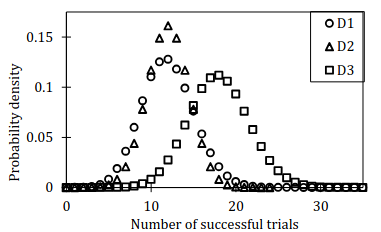
\includegraphics[width=0.6\columnwidth]{figs/pic8.png} 
   \caption*{}
  \label{fig:Q36}
\end{figure}

Each of the plotted distributions corresponds to a unique pair of $\brak{n, p}$ values, where, $n$ is the number of trials and $p$ is the probability of success in a trial. Three sets of $\brak{n, p}$ values are provided in the table.

\hfill{\brak{\text{GATE PE 2018}}}

\begin{center}
\begin{tabular}{|c|c|}
\hline
Set & (n, p) \\
\hline
I & (60, 0.3) \\
II & (60, 0.2) \\
III & (24, 0.5) \\
\hline
\end{tabular}
\end{center}

Pick the correct match between the $\brak{n, p}$ set and the plotted distribution.

\begin{enumerate}
\begin{multicols}{2}
\item Set I - D1, Set II - D2, Set III - D3 \item Set I - D3, Set II - D1, Set III - D2 \item Set I - D2, Set II - D3, Set III - D1 \item Set I - D2, Set II - D1, Set III - D3
\end{multicols}
\end{enumerate}

\item Which of the following statements are true about Natural Gas Hydrates?

\hfill{\brak{\text{GATE PE 2018}}}

\noindent
Natural gas hydrates:

\begin{enumerate}
\item are formed under low temperature and high pressure.
\item can store approximately 160 m$^3$ of gas per m$^3$ of hydrate at $25{\degree}C$ and 1 atm.
\item formation is an endothermic process.
\item are potential sources of methane.
\end{enumerate}

\begin{enumerate} 
\begin{multicols}{2}
\item Only II, III \& IV \item Only I, II \& III
\item Only I, II \& IV  \item Only I, III \& IV 
\end{multicols}
\end{enumerate}

\pagebreak

\item $P_{wf}$ \brak{\text{bottom-hole well flowing pressure}} vs. Q \brak{\text{flow rate}} plots show the inflow performance relation \brak{IPR} and vertical lift performance \brak{VLP} curves. Figure I shows VLP curves for two well head pressures $P_{hw1}$ and $P_{hw2}$. Figure II shows VLP curves for two well diameters $D_1$ and $D_2$. Which one of the following statements is true?

\hfill{\brak{\text{GATE PE 2018}}}

\begin{figure}[h!]
  \centering
  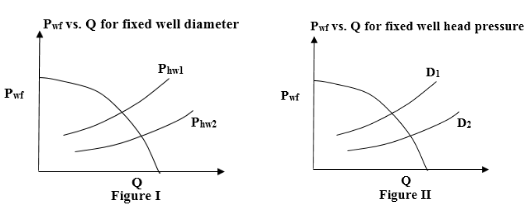
\includegraphics[width=0.8\columnwidth]{figs/pic9.png} 
   \caption*{}
  \label{fig:Q38}
\end{figure}

\begin{enumerate}
\begin{multicols}{2}	
\item $P_{hw1} > P_{hw2}$ and $D_1 < D_2$ \item $P_{hw1} > P_{hw2}$ and $D_1 > D_2$
\item $P_{hw1} < P_{hw2}$ and $D_1<D_2$ \item  $P_{hw1} < P_{hw2}$ and $D_1 > D_2$
\end{multicols}
\end{enumerate}

\item Match the following: 

\hfill{\brak{\text{GATE PE 2018}}}

\begin{tabular}{ll}
P. Weber Number      & I. Ratio of inertial force to viscous force \\
Q. Froude Number     & II. Ratio of convective heat transfer to conductive heat transfer \\
R. Reynolds number   & III. Ratio of inertial force to interfacial force \\
S. Nusselt number    & IV. Ratio of inertial force to gravitational force \\\\
\end{tabular}

\begin{enumerate} 
\begin{multicols}{2}
\item P-III, Q-IV, R-I, S-II \item P-III, Q-II, R-I, S-IV 
\item P-II, Q-III, R-IV, S-I \item P-IV, Q-III, R-I, S-II 
\end{multicols}
\end{enumerate}

\item A dilute mixture of coal and sand particles, both of diameter $100m$ and densities 1800~kg/m$^3$ and 2600~kg/m$^3$, respectively, is to be classified by elutriation technique using water \brak{\text{density 1000~kg/m$^3$, viscosity $10^{-3}$~Pa$\cdot$s}}. Assuming Stokes law is applicable, the minimum settling velocity of the particles in the mixture is \brak{\text{g = 9.81~m/s$^2$}}: 

\hfill{\brak{\text{GATE PE 2018}}}

\begin{enumerate}
\begin{multicols}{2}
\item 4.36 $\times$ 10$^{-3}$ m/s \item 8.72 $\times$ 10$^{-3}$ m/s 
\item 2.18 $\times$ 10$^{-3}$ m/s \item 1.29 $\times$ 10$^{-3}$ m/s 
\end{multicols}
\end{enumerate}

\pagebreak

\item Oil flow rate and flowing bottom-hole pressure \brak{FBHP} recorded with time during a multi-
rate well test are shown.

\hfill{\brak{\text{GATE PE 2018}}}

\begin{figure}[h!]
  \centering
  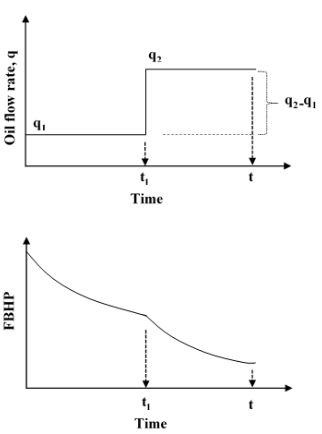
\includegraphics[width=0.4\columnwidth]{figs/pic10.png} 
  \caption*{}
  \label{fig:Q41}
\end{figure}

Let $k$ is the reservoir permeability, $h$ is the formation thickness and $\mu$ is the viscosity of the oil. $\Delta P_D(t)$ is constant-rate dimensionless pressure drop as a function of time. The total pressure drop till time, $t$, where $t > t_1$, will be: 

\hfill{\brak{\text{GATE PE 2018}}}

\begin{enumerate}
\begin{multicols}{2}
\item $\dfrac{q_1 \mu}{2 \pi k h} \Delta P_D(t) + \dfrac{(q_2 - q_1) \mu}{2 \pi k h} \Delta P_D(t - t_1)$ 
\item $\dfrac{q_1 \mu}{2 \pi k h} \Delta P_D(t_1) + \dfrac{(q_2 - q_1) \mu}{2 \pi k h} \Delta P_D(t - t_1)$
\item $\dfrac{q_1 \mu}{2 \pi k h} \Delta P_D(t) + \dfrac{q_2 \mu}{2 \pi k h} \Delta P_D(t - t_1)$
\item $\dfrac{q_1 \mu}{2 \pi k h} \Delta P_D(t_1) + \dfrac{q_2 \mu}{2 \pi k h} \Delta P_D(t)$
\end{multicols}
\end{enumerate}

\item Which one of the following options presents the correct combination? 

\hfill{\brak{\text{GATE PE 2018}}}

\begin{tabular}{ll}
P. Reservoir limit test         & I. Communication between wells \\
Q. Modified isochronal test     & II. Ideally zero flowing bottom hole pressure \\
R. Interference test            & III. Extended drawdown test \\
S. Absolute open flow potential & IV. Drawdown and build-up test of equal duration\\ 
\end{tabular}

\begin{enumerate}
\begin{multicols}{2}
\item P-II, Q-III, R-I, S-IV \item P-IV, Q-I, R-III, S-II 
\item P-III, Q-IV, R-I, S-II \item P-I, Q-III, R-IV, S-II 
\end{multicols}
\end{enumerate}

\pagebreak

\item Which one of the following options presents the correct combination? 

\hfill{\brak{\text{GATE PE 2018}}}

\begin{tabular}{ll}
P. Roller Cone bits    & I. Long and widely spaced teeth \\
Q. PDC bits            & II. Journal (Pin) angle \\
R. Soft formation      & III. Short and wider teeth \\
S. Hard formation      & IV. Size of the cutting \\
T. Back rake angle     & V. 1400$^\circ$C and 6$\times$10$^5$ psi \\
\end{tabular}

\begin{enumerate} 
\begin{multicols}{2}
\item P-II, Q-V, R-I, S-III, T-IV \item P-III, Q-IV, R-I, S-II, T-V \\
\item P-III, Q-II, R-IV, S-I, T-V \item P-II, Q-V, R-III, S-I, T-IV \\
\end{multicols}
\end{enumerate}

\item Primary and secondary indicators of kick in a well where the indicators are: 

\hfill{\brak{\text{GATE PE 2018}}}

\begin{enumerate}
\item flow rate increase,
\item gas, oil or water-cut muds,
\item pit volume increase,
\item flowing well with mud pump shut-off,
\item reduction in drill-pipe weight,
\item drilling break.
\end{enumerate}

\noindent
Which one of the following presents the correct combination?


\begin{enumerate} 
\item Primary\brak{1, 3, 5} and Secondary\brak{2, 4, 6}
\item Primary\brak{1, 2, 3} and Secondary\brak{4, 5, 6} 
\item Primary\brak{1, 2, 4} and Secondary\brak{3, 5, 6} 
\item Primary\brak{1, 3, 4} and Secondary\brak{2, 5, 6} 
\end{enumerate}

\item Relative permeability curve for the two rock types \brak{\text{X: solid line and Y: dashed line}} are shown in the diagram, where Sw is the fractional water saturation.Which one of the following statements is correct about wettability and consolidated nature of the two rock types?

\hfill{\brak{\text{GATE PE 2018}}}

\begin{figure}[h!]
  \centering
  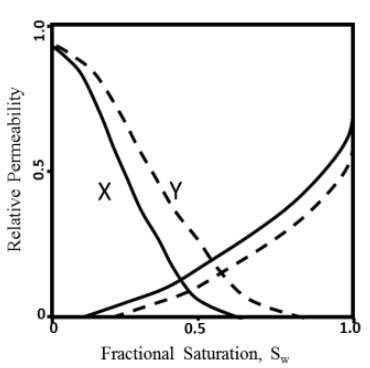
\includegraphics[width=0.3\columnwidth]{figs/pic11.png} 
   \caption*{}
  \label{fig:Q45}
\end{figure}

\begin{enumerate} 
\item X is more consolidated and mixed wet, Y is less consolidated and water wet
\item X is more consolidated and water wet, Y is less consolidated and mixed wet
\item X is less consolidated and mixed wet, Y is more consolidated and water wet
\item X is less consolidated and water wet, Y is more consolidated and mixed wet\\
\end{enumerate}

\pagebreak

\item Which one of the following options presents correct combinations of exploration methods with their respective frequency of operation? 

\hfill{\brak{\text{GATE PE 2018}}}

\begin{tabular}{ll}
P. Seismic               & I. ~$10^6$ Hz \\
Q. Sonic                 & II. ~$10^2$ Hz \\
R. Controlled Source EM & III. ~$10^4$ Hz \\
S. Ultrasonic            & IV. ~1 Hz \\
\end{tabular}

\begin{enumerate} 
\begin{multicols}{2}
\item P-IV, Q-II, R-I, S-III \item P-II, Q-III, R-IV, S-I \\
\item P-II, Q-I, R-IV, S-III \item P-IV, Q-I, R-II, S-III \\
\end{multicols}
\end{enumerate}

\item Which one of the following options presents the correct combinations? 

\hfill{\brak{\text{GATE PE 2018}}}

\begin{tabular}{ll}
P. Borisov's  & I. Critical rate correlation in vertical wells with coning \\
Q. Schols'    & II. Horizontal well performance relation \\
R. Efros'     & III. Vertical well performance relation \\
S. Wiggins'   & IV. Critical rate correlation in horizontal wells with coning 
\end{tabular}

\begin{enumerate} 
\begin{multicols}{2}
\item P-II, Q-IV, R-I, S-III \item P-IV, Q-III, R-II, S-I \\
\item P-IV, Q-II, R-III, S-I \item P-II, Q-I, R-IV, S-III \\
\end{multicols}
\end{enumerate}

\item Which one of the following options represents the typical sequence of applying cut-offs for pay zone identification in a conventional reservoir? 

\hfill{\brak{\text{GATE PE 2018}}}

\begin{enumerate} 
\begin{multicols}{2}
\item porosity, saturation, shale \item porosity, permeability, saturation \\
\item shale, porosity, saturation \item shale, porosity, permeability \\
\end{multicols}
\end{enumerate}

\item Which one of the following options represents the correct sequence of arrival of acoustic wave energy recorded in a sonic log? 

\hfill{\brak{\text{GATE PE 2018}}}

\begin{enumerate}
\begin{multicols}{2}
\item shear, surface, compressional  \item compressional, shear, surface \\ 
\item surface, shear, compressional  \item compressional, surface, shear \\
\end{multicols}
\end{enumerate}

\item The variation of the amount of salt in a tank with time is given by, 

\hfill{\brak{\text{GATE PE 2018}}}

\begin{align*} 
\frac{dx}{dt} + 0.025x = 20
\end{align*}

where, $x$ is the amount of salt in kg and $t$ is the time in minutes. Given that there is no salt in the tank initially, the time at which the amount of salt increases to 200 kg is \underline{\hspace{2cm}} minutes. \brak{\text{rounded-off to two decimal places}}

\pagebreak

\item Solve the given differential equation using the 2\textsuperscript{nd} order Runge-Kutta \brak{RK2} method: 

\hfill{\brak{\text{GATE PE 2018}}}

\begin{align*} 
\frac{dy}{dt} = t - \sqrt{y} \quad ; \quad \text{Initial condition: } y(0) = 4
\end{align*}

Use the following form of RK2 method with an integration step-size, $h = 0.5$:
\begin{align*} 
k_1 = f(t_i, y_i) \quad ; \quad k_2 = f(t_i + 0.5h, y_i + 0.5k_1 h) 
\end{align*}
\begin{align*}
y_{i+1} = y_i + k_2 h 
\end{align*}
The value of $y(t = 0.5) = \underline{\hspace{2cm}}$. \brak{\text{rounded-off to two decimal places}}\\\\

\item A box contains 100 balls of same size, of which, 25 are black and 75 are white. Out of 25 black balls, 5 have a red dot. A trial consists of randomly picking a ball and putting it back in the same box, i.e., sampling is done with replacement. Two such trials are done. The conditional probability that no black ball with a red dot is picked given that at least one black ball is picked, is \underline{\hspace{2cm}}. \brak{\text{in fraction rounded-off to two decimal places}} 

\hfill{\brak{\text{GATE PE 2018}}}

\item A cylindrical pipeline of length 30 km is transporting naphtha. Pressure sensors are attached along pipe length to detect leaks. Under steady-state, leak-free operation, there is a linear pressure drop along the length $z$ of the pipeline. If a leak occurs, the pressure profile develops a kink at the leak point $z_{\text{leak}}$.


Assume that there is only one leak-point ($4~\text{km} < z_{\text{leak}} < 27~\text{km}$) and a new steady-state is reached. The steady-state pressure measurements at four locations along the pipe-length are provided in the table. The location of the leak-point using the \textit{gradient intersection method} is \underline{\hspace{2cm}} km. \brak{\text{rounded-off to two decimal places}} 

\hfill{\brak{\text{GATE PE 2018}}}

\begin{tabular}{|c|c|}
\hline
$z$ (km) & Pressure \\
\hline
0 & $p_0$ \\
4 & $0.84p_0$ \\
27 & $0.31p_0$ \\
30 & $0.25p_0$ \\
\hline
\end{tabular}

\pagebreak

\item A dry core was subjected to the mercury injection test in the laboratory. Following are the related details:  

\begin{enumerate}
\item Average formation porosity = 0.2 
\item Formation volume factor, $B_o = 1.2$ reservoir-bbl/STB  
\item Oil API$^\circ$ = 32, Specific gravity of water = 1.1 
\item Hydrostatic gradient = 0.433 psi/ft  
\item $(\sigma_{OW} \cos \theta)_{res}$ = 26 dyne/cm, where $\sigma_{OW}$ is the oil-water interfacial tension and $\theta$ is the contact angle 
\item $(\sigma_{AM} \cos \theta)_{lab}$ = 367 dyne/cm, where $\sigma_{AM}$ is air- mercury interfacial tension and $\theta$ is the contact angle 
\item Average drainage area = 80 acres 
\end{enumerate}

(1 acre-ft = 7758 bbl) \\ 

The Table shows the laboratory data for capillary pressure at different mercury saturations.


\begin{tabular}{|c|c|}
\hline
$P_c$ (psia) & Mercury saturation ($S_{Hg}$) \\
\hline
10 & 0.0075 \\
17 & 0.25 \\
30 & 0.50 \\
108 & 0.70 \\
2000 & 0.85 \\
\hline
\end{tabular}


$P_c = \frac{2\sigma \cos \theta}{r}$ and the average water saturation $\brak{S_W}$ for the productive column is 0.25. The Original Oil in Place \brak{OOIP} in the productive column where $S_W \leq 0.5$ is \underline{\hspace{2cm}} MMSTB. \brak{\text{rounded-off to two decimal places}} 

\hfill{\brak{\text{GATE PE 2018}}}


\item A well is drilled with water based mud. The water saturation in the completely flushed zone (no formation fluid residual) is given by, 
\begin{align*}
S_{xo} = \left( \frac{a}{\phi^2} \times \frac{R_{mf}}{R_{xo}} \right)^{1/2}
\end{align*}
where, $R_{mf}$ and $R_{xo}$ are the mud filtrate resistivity and flushed zone resistivity, respectively. Use, $a = 1.0$ and $R_{xo} = 25 R_{mf}$. 
The calculated porosity $\brak{\phi}$ of the formation is \underline{\hspace{2cm}}. \brak{\text{in fraction rounded-off to two decimal places}} 

\hfill{\brak{\text{GATE PE 2018}}}

\item An oil well is tested at a flow rate $\brak{Q}$ of 50 BOPD. The bottom hole flowing pressure $\brak{P_{wf}}$ is 500 psia. The shut-in pressure is 1000 psia. If $P_{wf}$ is lowered to 300 psia and assuming the Vogel's correlation holds, the estimated flow rate in the oil well is \underline{\hspace{2cm}} BOPD \brak{\text{rounded-off to two decimal places}}. The Vogel's correlation is:

\begin{align*}
\frac{Q}{Q_{max}} = 1 - 0.2\left(\frac{P_{wf}}{\bar{P}}\right) - 0.8\left(\frac{P_{wf}}{\bar{P}}\right)^2 
\end{align*}
\hfill{\brak{\text{GATE PE 2018}}}
\pagebreak

\item Using Miller, Dyes and Hutchinson \brak{MDH} method, the skin factor of an oil well is found to be $s = -3.5$. \\ 

The reservoir and fluid properties are: 

\begin{itemize}
\item Formation porosity is 0.20
\item Total compressibility is $2.5 \times 10^{-5}$ psia$^{-1}$
\item Oil viscosity is 1.5 cP
\item Wellbore radius is 0.5 ft
\item Flowing bottom hole pressure at $\Delta t = 0$ is 2830 psia
\item Shut in pressure at $\Delta t = 1$ hr $\brak{P_{\Delta t=1hr}}$ is 3000 psia
\item Slope of middle time region \brak{MTR} line in MDH plot is 190 psia/cycle
\end{itemize}

The permeability of the reservoir is \underline{\hspace{2cm}} mD. \brak{\text{rounded-off to two decimal places}} 

\hfill{\brak{\text{GATE PE 2018}}}

\item An oil well \brak{\text{producing under expansion drive only}} in a reservoir is subjected to two pressure build-up tests. The average formation thickness of the reservoir is 13 ft, the total compressibility is $1\times10^{-5}$ psia$^{-1}$, and porosity is 0.2. The average formation volume factor of oil is 1.3 reservoir-bbl/STB. Average reservoir pressure during the first test and the second test was found to be 3500 psia and 3200 psia, respectively. \\ 
If the oil produced between the two pressure build-up tests in 180 days is 250 STB/day, the area of the reservoir is \underline{\hspace{2cm}} acres. \brak{\text{rounded-off to two decimal places}} \\ 
\brak{\text{Use: 1 acre = 43560 ft$^2$, 1 bbl = 5.615 ft$^3$}} 

\hfill{\brak{\text{GATE PE 2018}}}

\item A well in a very large reservoir has a wellbore radius of 10 cm. The sandstone, with a porosity of 0.25 and 12\% \brak{\text{by grain volume}} calcite $\brak{CaCO_3}$, is to be acidized with a preflush \brak{\text{HCl solution}} so as to dissolve all the calcite up to a distance of 1 m from the wellbore. 1 m$^3$ of preflush is able to dissolve 0.082 m$^3$ CaCO$_3$. Assume that the reaction between HCl and CaCO$_3$ is instantaneous. 

The minimum preflush volume required per meter of the formation thickness is \underline{\hspace{2cm}} m$^3$. \brak{\text{rounded-off to two decimal places}} 

\hfill{\brak{\text{GATE PE 2018}}}

\item At a particular temperature, the vapour pressure of benzene and toluene are 4 atm and 1.2 atm, respectively. The composition of the liquid at equilibrium is 0.5 moles of benzene and 0.5 moles of toluene. Assuming ideal gas and ideal solution, the equilibrium vapour phase mole fraction of benzene is \underline{\hspace{2cm}}. \brak{\text{rounded-off to two decimal places}} 

\hfill{\brak{\text{GATE PE 2018}}}

\item Saturated steam at 0.7 atm and 90$^\circ$C condenses on a vertical pipe of 2 cm outside diameter and 40 cm length. The average condensation heat transfer coefficient on the tube is 12000 W/m$^2$K. The outside surface temperature of the pipe is maintained constant at 85$^\circ$C. \\ 
The enthalpy values for saturated steam and condensate are 2660 kJ/kg and 375 kJ/kg, respectively. The rate of steam condensation is \underline{\hspace{2cm}} kg/h.\\
\brak{\text{rounded-off to two decimal places}} 

\hfill{\brak{\text{GATE PE 2018}}}

\item Oil is being transported between two reservoirs with the help of three parallel pipes at steady state. The diameters of these pipes are 2 cm, 3 cm and 4 cm, respectively. The pipes are equal in length and the flow is laminar. The discharge through the 4 cm diameter pipe is 50 liters/s. The discharge through the 2 cm diameter pipe is \underline{\hspace{2cm}} liters/s. \brak{\text{rounded-off to two decimal places}} 

\hfill{\brak{\text{GATE PE 2018}}}

\pagebreak

\item A driller finds an oil reservoir with a gas cap starting at a depth of 1000 m from the surface. The gas-oil contact was found at 1100 m depth and water-oil contact was found at 1300 m depth. The water pressure in the aquifer below the oil zone varies with depth from the surface \brak{\text{$h$, in meters}} as, $P = h \times 10^4$ Pa. The density of the oil is 900 kg/m$^3$ and that of gas is 5 kg/m$^3$ at the reservoir condition. The minimum density of the mud needed to stop the gas kick when the driller reaches at the top of the gas cap is \underline{\hspace{2cm}} kg/m$^3$. \brak{\text{rounded-off to two decimal places. Use $g = 9.81$ m/s$^2$}} 

\hfill{\brak{\text{GATE PE 2018}}}

\item The viscosity, $\mu$ \brak{\text{in Pa.s}} of a power law fluid as a function of shear rate, $\dot{\gamma}$ \brak{\text{in s$^{-1}$}} is given by the following relation: 

\begin{align*} 
\mu = \frac{1}{2} |\dot{\gamma}| 
\end{align*}

This power law fluid lies between two infinitely large horizontal parallel plates separated by a distance $\brak{h}$ of 10$^{-3}$ m. The top plate is moving horizontally at a velocity $\brak{v}$ of 10$^{-3}$ m/s and the bottom plate is held stationary. Assuming laminar flow and neglecting gravity, the absolute value of steady-state shear stress acting on the bottom plate is \underline{\hspace{2cm}} Pa. \brak{\text{rounded-off to two decimal places}} 

\hfill{\brak{\text{GATE PE 2018}}}

\item A heterogeneous rectangular rock of cross-sectional area 1 m2 perpendicular to the flow is
being flooded by water to measure the effective permeability from cross-section AA' to
cross-section CC'.

\hfill{\brak{\text{GATE PE 2018}}}\\\\

\begin{figure}[h!]
  \centering
  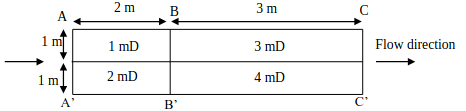
\includegraphics[width=0.8\columnwidth]{figs/pic12.png} 
   \caption*{}
  \label{fig:Q65}
\end{figure}

The pressure at the cross-sections AA', BB', and CC' is 2 bar, 1.5 bar, and 1 bar,
respectively. The permeability in mili-Darcy and lengths AB and BC in meters are given in
the figure. The effective permeability of the rock from AA' to CC' is \underline{\hspace{4cm}}mD. 
\brak{\text{rounded-off to two decimal places}}\\\\



\begin{center}
	{\LARGE \textbf{END OF THE QUESTION PAPER}}
\end{center}

\end{enumerate}

\end{document}
